\documentclass[output=paper]{langscibook} 
\ChapterDOI{10.5281/zenodo.5578838}
\author{Stephen Nichols\affiliation{University of Manchester}}
\title{Asymmetries in vowel-pair frequencies and height harmony in Bantu}
\abstract{In this paper, I present an exploration of vowel-pair frequencies in the nouns of six five-vowel Bantu languages and discuss their relationship with those alternations seen in verbs due to height harmony. Of particular interest is the disparity in the frequencies of two vowel pairs disagreeing in height, specifically [e.i] and [o.u], both between themselves and with the corresponding pairs which agree in height, namely [e.e] and [o.o]. The results show that while both [e.e] and [o.o] are over-represented, [e.i] and [o.u] are generally under-represented. In addition to this, [o.u] is consistently less frequent than [e.i] and the difference in representation between [o.o] and [o.u] is larger than between [e.e.] and [e.i].}

\begin{document}
\SetupAffiliations{mark style=none}
\maketitle

\section{Introduction}\label{sec:nichols:introduction}

It is well documented in the literature that vowel height harmony as instantiated in the Bantu languages is most often asymmetric with respect to rounding and/or backness and also often gives rise to alternations only in verbs (see e.g. \citealt{Hyman99}; for more see also \sectref{sec:nichols:background}). In this paper, I present an exploration of vowel-pair frequencies in nouns in six five-vowel Bantu languages -- Chewa, Kalanga, Lozi, Makhuwa, Pende and Yao -- and also discuss the results in the context of the system of height harmony found in each language. For reasons of space, I limit myself to the discussion of just four vowel pairs that are of particular interest, namely [e.e]--[e.i] and [o.o]--[o.u].

The results reveal that, in nouns, the two pairs that agree in height -- [e.e] and [o.o] -- consistently occur more frequently than their counterparts that do not agree in height -- [e.i] and [o.u], with the differences between [o.o] and [o.u] being starker than those between [e.e] and [e.i]. This is despite the fact that, in these languages, active alternations are only seen in verbs. Moreover, there is a trend for the pairs [e.i] and [o.u] to be relatively under-represented compared to [e.e] and [o.o] across the sample. The results also show that, though both occur at below-expected levels, the rounded back pair [o.u] is less frequent than [e.i], even taking into account the relative frequencies of the component vowels according to position.

Previous work such as \citet{Archangeli12b} has also noted the under-representation in nouns of pairs repaired by alternations in verbs.\footnote{In addition, \citet{VHCalc} found that, in Swahili, verbs were highly height harmonic and that nouns were also generally height harmonic at an above-chance rate.} However, the difference between the two non-harmonic pairs [e.i] and [o.u] is not remarked upon, though it can be seen in their data (see e.g. Figure~2). In addition to this, the sample used by \citet{Archangeli12b} looked only at canonical five-vowel languages.

In this chapter, I examine three non-canonical languages, including two in which alternations of front vowels in verbs do not occur. In both languages lacking front-vowel alternations, [e.e] and [o.o] are more represented than [e.i] and [o.u] respectively; however, [e.e] is found only marginally more than [e.i] in Lozi.

In sum, though alternations are only observed in verbs, the results show that there is nevertheless a preference in nouns for those pairs that agree in height.

\section{Background}\label{sec:nichols:background}

This exploration of vowel-pair frequencies considers a sample of six five-vowel\footnote{That is, languages having the vowel phoneme inventory /i u e o a/.} Bantu languages. The details of these languages are provided in \tabref{tab:nichols:sample} before vowel height harmony in particular is discussed further below.

\begin{table}
\caption{The six-language sample of five-vowel Bantu languages\label{tab:nichols:sample}}
\fittable{\begin{tabular}{llllr}
\lsptoprule
Language & Guthrie code & Harmony system & Data source & Size\\
\midrule
Chewa & M.31b & canonical & \citet{Mtenje01} & 24,076 \\
Kalanga & S.16 & canonical & \citet{Mathangwane94} & 8,505 \\
Lozi & K.21 & back only & \citet{Jalla82CBOLD} & 49,981 \\
Makhuwa & P.31 & back only & \citet{Kisseberth96} & 29,802 \\
Pende & L.11 & quasi-canonical & \citet{Gusimana72CBOLD} & 38,385 \\
Yao & P.21 & canonical & \citet{Ngunga01} & 25,954 \\
\lspbottomrule
\end{tabular}}
\end{table}

As can be seen from \tabref{tab:nichols:sample}, each language possesses a certain harmony system, with three different systems being represented in this sample. Vowel height harmony writ large is a widespread trait among the Bantu languages (\citealt[236]{Hyman99}, \citeyear[46--47]{Hyman03}; \citealt[7]{Nurse03a}; \citealt[\S{1}]{Odden15}). In five-vowel languages, such as Shona (S.11; \citealt{Beckman97}), this often leads to active alternations only in verbal suffixes, excluding final vowels. Indeed, \citet[38]{Beckman97} comments that ``[t]he distributional generalisations which apply to height features in Shona verbs apparently do not hold of Shona nouns'' and that ``vowel height in nouns is contrastive outside of the root-initial syllable''. In other cases, however, static generalisations analogous to the alternations found in verbs may also be seen within a majority of noun stems.\footnote{Note also that there are Bantu languages that show alternations in nouns due to vowel harmony, such as noun class prefixes in seven-vowel Koyo (C.24; see e.g. \citealt[240]{Hyman99}).} This has previously been said, for example, of Chewa (\citealt{Scullen92} in \citealt[75]{Downing17}).

The commonest variant of height harmony is the so-called ``canonical'' pattern \citep[after][238]{Hyman99}. In five-vowel languages that possess canonical height harmony -- such as Chewa, Kalanga and Yao -- high vowels are lowered to mid vowels by preceding mid vowels whereas the low vowel /a/ neither triggers nor undergoes lowering and is opaque. In addition, as mentioned in \sectref{sec:nichols:introduction}, canonical height harmony is asymmetric with respect to rounding and/or backness. That is, /i/ is lowered to [e] after both /e/ and /o/ whereas /u/ is lowered to [o] only following /o/. In at least purely descriptive terms then, it is useful to talk of both front and back height harmony.

Canonical height harmony is exemplified in \REF{ex:nichols:chewa-f} and \REF{ex:nichols:chewa-b} with Chewa data taken from \citet[71--72]{Downing17}.\footnote{For the sake of the simplicity of exposition, the infinitive prefix, tone and effects such as penultimate lengthening have been omitted in the examples provided in this section.}

\begin{multicols}{2}
\ea \label{ex:nichols:chewa-f}
\ea \textit{-phikila} `to cook for'
\ex \textit{-khutila} `to be satisfied with'
\ex \textit{-tsekela} `to close for'
\ex \textit{-gonela} `to sleep on'
\ex \textit{-valila} `to put on'
\z
%
\ex \label{ex:nichols:chewa-b}
\ea \textit{-pitikula} `to overturn'
\ex \textit{-funthula} `to loosen'
\ex \textit{-tsekula} `to open'
\ex \textit{-wonjola} `to spring a trap'
\ex \textit{-sankula} `to choose out from'
\z
\z
\end{multicols}

The majority of work on height harmony in five-vowel Bantu languages has focused on this pattern. Indeed, Chewa has been an especially popular case study (see e.g. \citealt{Mtenje85, Scullen92, Harris94, Harris97, Sandstedt19}). A selection of other well-known languages exhibiting this are Bemba (M.42; \citealt{Kula00a, Kula02}), Luganda (E.15; \citealt{Katamba84}), Shona (S.11; \citealt{Beckman97}) and Swahili (G.42; \citealt{Marten96, Marten97}).

The ``quasi-canonical'' variety of harmony found in Pende differs from the pattern found in Chewa in just one instance. Specifically, in front height harmony, mid [e] is found after the low vowel /a/ rather than high [i]. This is illustrated in \REF{ex:nichols:pende-f} and \REF{ex:nichols:pende-b} with examples from \citet{Gusimana72CBOLD}.

\begin{multicols}{2}
\ea \label{ex:nichols:pende-f}
\ea \textit{-shitila} `to close for'
\ex \textit{-tungila} `to build for'
\ex \textit{-bembela} `to leave for'
\ex \textit{-solela} `to clear [land] for'
\ex \textit{-talela} `to monitor for'
\z
%
\ex \label{ex:nichols:pende-b}
\ea \textit{-jitulula} `to untie'
\ex \textit{-kubula} `to collapse'
\ex \textit{-ketula} `to make a notch'
\ex \textit{-logola} `to pour out'
\ex \textit{-batula} `to cut off, detach'
\z
\z
\end{multicols}

The final two languages in the sample -- Lozi and Makhuwa -- lack front height harmony, as seen in \REF{ex:nichols:lozi-fh} and \REF{ex:nichols:lozi-fl} with Lozi data culled from \citet{Jalla82CBOLD}.

\begin{multicols}{2}
\ea \label{ex:nichols:lozi-fh}
\ea \textit{-pimisa} `to help avoid'
\ex \textit{-hupulisa} `to remind'
\ex \textit{-lembisa} `to put to shame'
\ex \textit{-longisa} `to help load'
\ex \textit{-tamisa} `to help tie'
\z
%
\ex \label{ex:nichols:lozi-fl}
\ea \textit{-bihela} `to report to'
\ex \textit{-fuluhela} `to paddle towards'
\ex \textit{-lemela} `to fell for'
\ex \textit{-shombotela} `to catch for'
\ex \textit{-shamela} `to urinate in'
\z
\z
\end{multicols}

They do, however, possess back height harmony. This is shown in \REF{ex:nichols:lozi-b}, with data once again coming from Lozi \citep{Jalla82CBOLD}.

\begin{multicols}{2}
\raggedcolumns
\ea \label{ex:nichols:lozi-b}
\ea \textit{-tinulula} `to undress'
\ex \textit{-lutulula} `to unthatch'
\ex \textit{-lekulula} `to resell'
\ex \textit{-notolola} `to unlock'
\ex \textit{-pakulula} `to unbolt'
\z
\z
\end{multicols}

\section{Methodology}

\subsection{Sources and pre-processing}

The data used in this study are taken from the Comparative Bantu Online Dictionary (CBOLD; citations for individual sources are given in \tabref{tab:nichols:sample}).\footnote{CBOLD is accessible via the following URL: \url{http://www.cbold.ish-lyon.cnrs.fr/}.} Each file was first hand-corrected for machine-readability. This consisted mainly of corrections to the tab-separation of columns and the addition of obvious missing line breaks, as well as certain minor corrections to obvious errors in transcriptions.\footnote{This was, however, conducted with all due caution in order to avoid introducing any potential bias into the results.} All subsequent processing and analysis was conducted using R \citep{R}.

It should be noted here that the data sets contain entries in citation forms with both simple and complex stems (for both nouns and verbs), including some instances of nouns derived from verbs. No morphemic analysis was conducted as the data sets did not indicate boundaries between roots within compounds, or between roots and suffixes. Thus, in this respect, the results presented in \sectref{sec:nichols:results} are based on vowel pairs that occur regardless of morphological context.

Each individual data set contained multiple columns of information, the total number of which varied slightly from language to language; however, only two columns contained in the raw data -- namely the word form itself and the part of speech -- were ultimately used. For each word, all content after the first space in the word column was removed to reduce contamination by non-target-language material (such as misaligned English-language definitions). This was then stripped of all non-alphabetic characters such as punctuation and numbers, and converted to lower case. Next, orthographic long vowels were shortened such that \textit{aa} became \textit{a} and so on. This was done as the feature of interest in this study is the quality rather than quantity of vowels. What's more, in certain cases long vowels may not be consistently transcribed, if at all. Finally, the number of part-of-speech labels for each data set was reduced to just three: verb, noun and other.\footnote{The data source for Lozi, for example, contained around 70 separate part-of-speech labels, largely distinguishing various different properties of verbs which were unnecessary for the present study. In addition to this, the Lozi dictionary was unique in that it also provided the perfective forms of verbs. In order to maintain a level of consistency across the entire sample, these were actively removed.} In the sections that follow, I concentrate predominantly on nouns.

\subsection{Processing and analysis}

The final data sets having been derived, the numbers of each unique vowel pho\-neme and pair were then computed, with each item retaining the part-of-speech label of the word in which it occurred. This yielded the raw count of each vowel phoneme and pair within a particular language. From this, the following within-language measures were derived: observed frequency, expected frequency, and observed--expected ratio.

The observed frequency of a vowel phoneme or pair is the quotient of the raw count of that particular phoneme or pair, divided by the total number of all vowel phonemes or pairs in the data set.

The expected frequency of a given vowel pair might have been derived simply by multiplying together the observed frequencies of the two constituent vowel phonemes of that pair without regard to which position in the pair the two vowels occur.\footnote{Of course, the two component vowels of a pair may or may not be the same as one another.} However, as noted in \citet{Archangeli12a, Archangeli12b}, due to, for example, morphological bias, the same vowel may not necessarily be found equiprobably in both positions and so, in order to take this into account, separate observed proportions were calculated for each vowel in both first and second position, which were then multiplied together to give the expected frequency of each pair.

The observed--expected ratio of a pair is the quotient of the observed frequency of that pair divided by its expected frequency. This is used as a gauge of the level of representation. A ratio of around 1 indicates that the vowel pair occurs approximately as frequently as expected, less than 1 that it is less frequent than expected (i.e. under-represented) and a ratio of more than 1 that it is more frequent than expected (i.e. over-represented). In addition to this, the magnitude of the ratio conveys the degree to which a pair is over- or under-represented within the language.

Lastly, note that, descriptive statistics were used rather than inferential statistics due to the small sample size of the current data set.

\section{Results}\label{sec:nichols:results}\largerpage[2]

Firstly, the raw counts in both nouns and verbs for each of the four vowel pairs of interest in this study -- i.e. [e.e], [e.i], [o.o] and [o.u] -- are shown in \autoref{fig:nichols:count}. These show that the pairs one would expect to be infrequent given the descriptions in \sectref{sec:nichols:background} do indeed occur at very low levels in verbs but that such low levels are not found for other pairs. Somewhat similarly, although generally found in higher numbers than in verbs, within each of the six languages in the sample [e.i] is found consistently less frequently than [e.e] in nouns. Likewise, [o.u], without exception, occurs less often in nouns than [o.o].

\begin{figure}[p]
\caption{Bar chart and figures for raw counts in nouns and verbs in all six languages}
\label{fig:nichols:count}
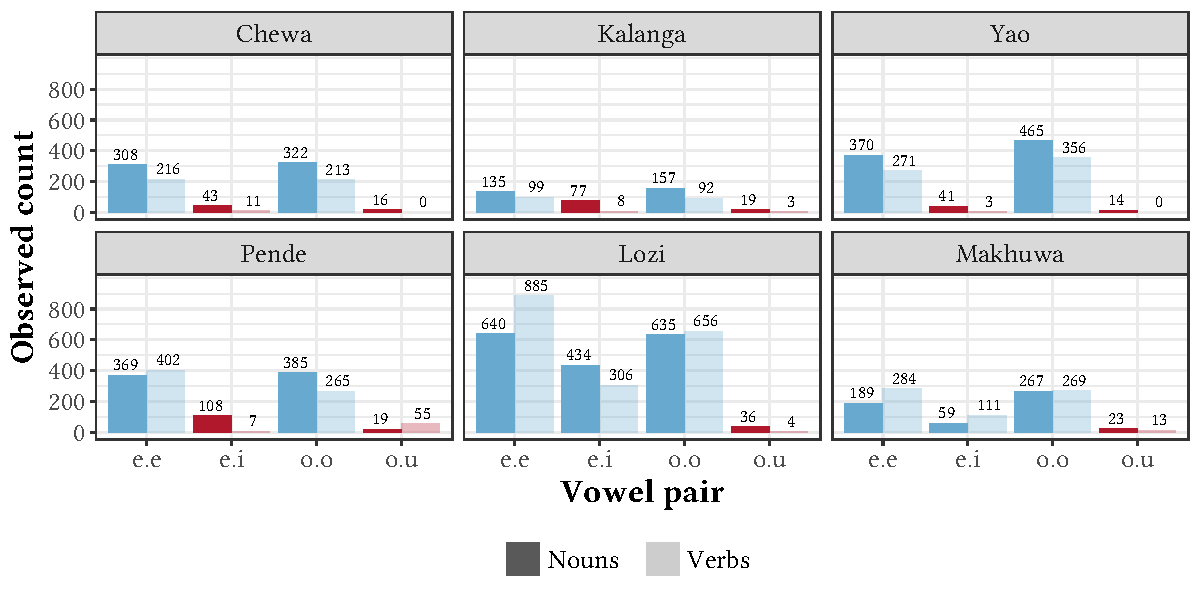
\includegraphics[width=1\textwidth]{./figures/nounverb.pdf}
\end{figure}

\begin{figure}[p]
\caption{Bar chart and figures for both observed and expected frequencies in nouns in all six languages}
\label{fig:nichols:realpred}
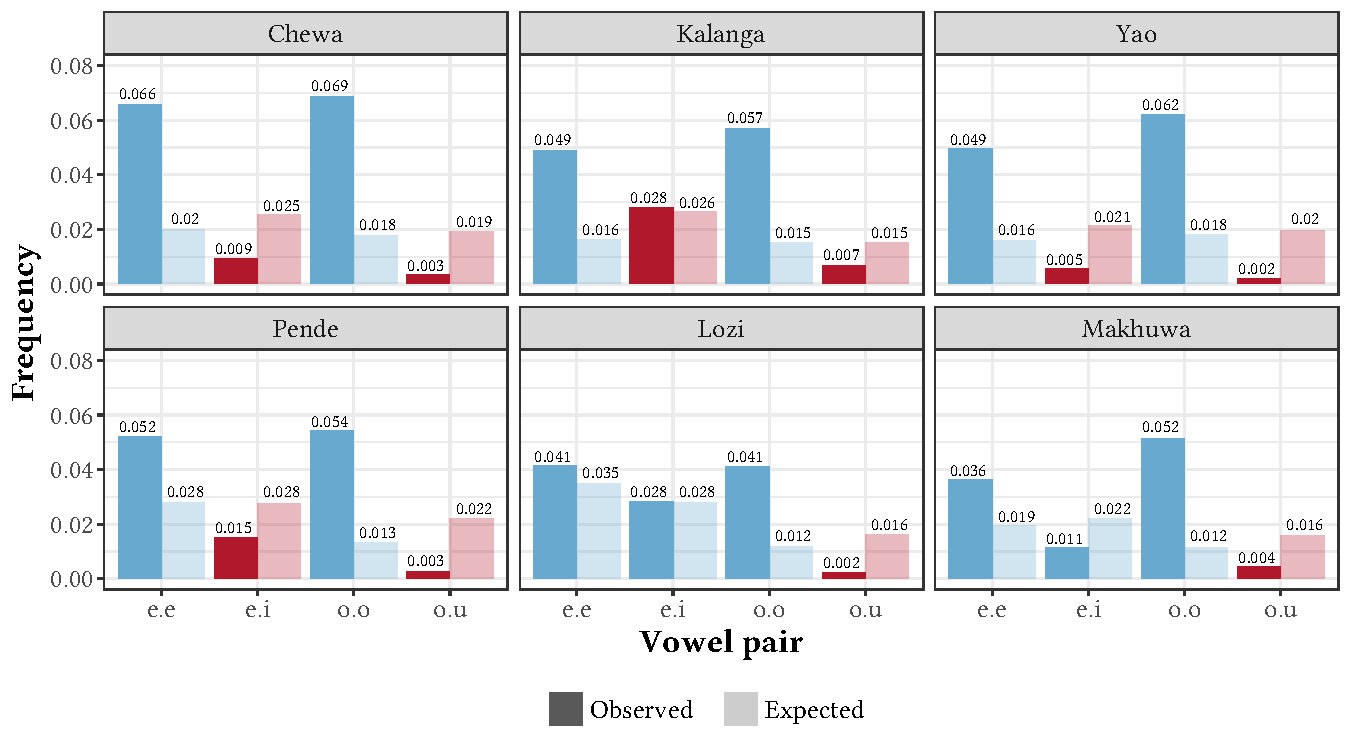
\includegraphics[width=1\textwidth]{./figures/realpred.pdf}
\end{figure}

Note that, in Figures \ref{fig:nichols:count}, \ref{fig:nichols:realpred} and \ref{fig:nichols:ratio}, pale blue is used to indicate those pairs that are assumed to be harmonic in that particular language and dark red signals those pairs assumed to be non-harmonic on the basis of alternations seen in verbal suffixes. This is used to illustrate how the harmony systems differ between languages with regard to these pairs. Thus, it can be seen that the above disparities between pairs are found in nouns irrespective of the harmony system of the particular language.

The differences described above in nouns on the basis of the raw count data are also reflected in the observed frequencies in nouns, given in \autoref{fig:nichols:realpred}. For the sake of completeness, alongside this, \autoref{fig:nichols:realpred} includes the expected frequencies for these same vowel pairs. This shows a different, much more evenly spread distribution (certain somewhat minor differences notwithstanding), indicating that these differences are not due simply to the relative frequencies in each vowel in the pair, even accounting for position.

Next, let us consider the corresponding observed--expected ratios in \autoref{fig:nichols:ratio}. Firstly, this shows that the pattern seen with the raw counts and observed frequencies remains. That is, in every language, the observed--expected ratios for [e.e] and [o.o] are larger than those for [e.i] and [o.u] respectively (however, for Lozi this difference is only slight).

Secondly, those pairs that agree in height -- i.e. [e.e] and [o.o] -- consistently occur at expected or higher-than-expected levels whereas those pairs that disagree in height -- i.e [e.i] and [o.u] -- are found at much lower levels than would be anticipated in all but 2 out of 12 cases.

\begin{figure}
\caption{Bar chart and figures for observed--expected ratios in nouns in all six languages (the horizontal dashed line indicates a ratio of 1).}
\label{fig:nichols:ratio}
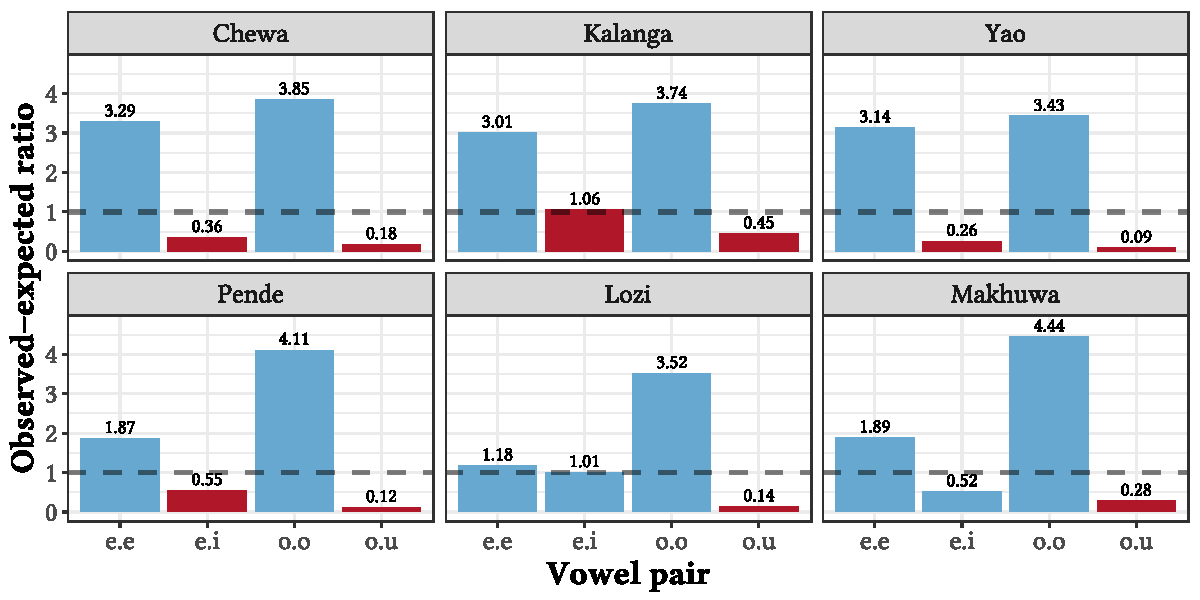
\includegraphics[width=1\textwidth]{./figures/ratio.pdf}
\end{figure}

For the sake of ease of comparison, and in order to reiterate and clarify certain points made above, the observed frequencies and observed--expected ratios of relevant pairwise comparisons are pooled and re-presented in Figures \ref{fig:nichols:eeei}, \ref{fig:nichols:oou} and \ref{fig:nichols:eiou}. Note, that, in these figures, the observed--expected ratios have been converted to log values in order to show over- and under-representation on the same scale, with positive values indicating over-representation and negative values under-representation.

\begin{figure}[p]
\caption{Boxplots of pooled observed frequencies (left) and log observed--expected ratios (right) in nouns for [e.e] and [e.i] only}
\label{fig:nichols:eeei}
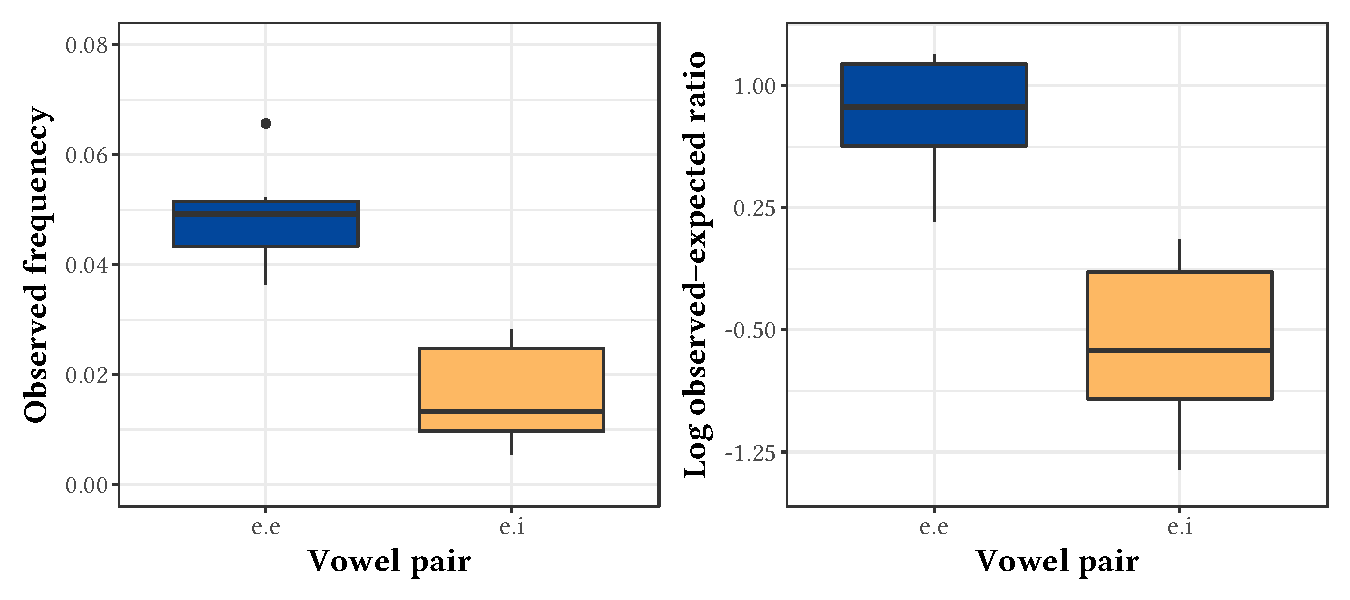
\includegraphics[width=0.875\textwidth]{./figures/eeei-log.pdf}
\end{figure}

\begin{figure}[p]
\caption{Boxplots of pooled observed frequencies (left) and log observed--expected ratios (right) in nouns for [o.o] and [o.u] only}
\label{fig:nichols:oou}
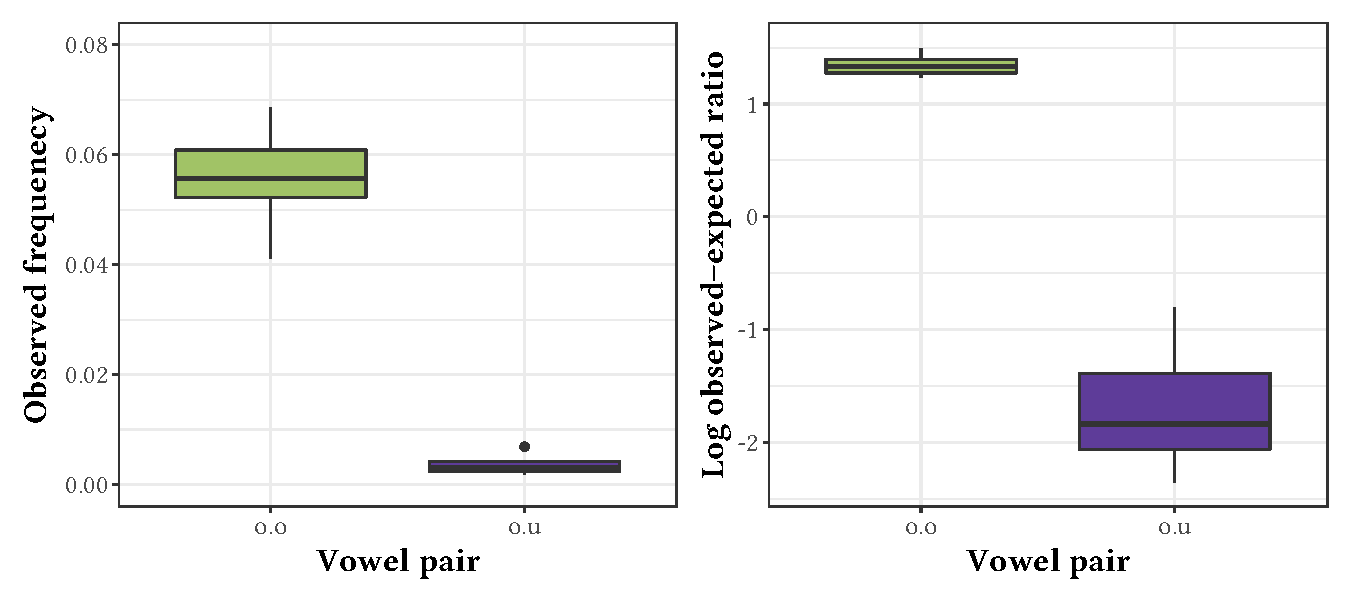
\includegraphics[width=0.875\textwidth]{./figures/ooou-log.pdf}
\end{figure}

\begin{figure}[p]
\caption{Boxplots of pooled observed frequencies (left) and log observed--expected ratios (right) in nouns for [e.i] and [o.u] only}
\label{fig:nichols:eiou}
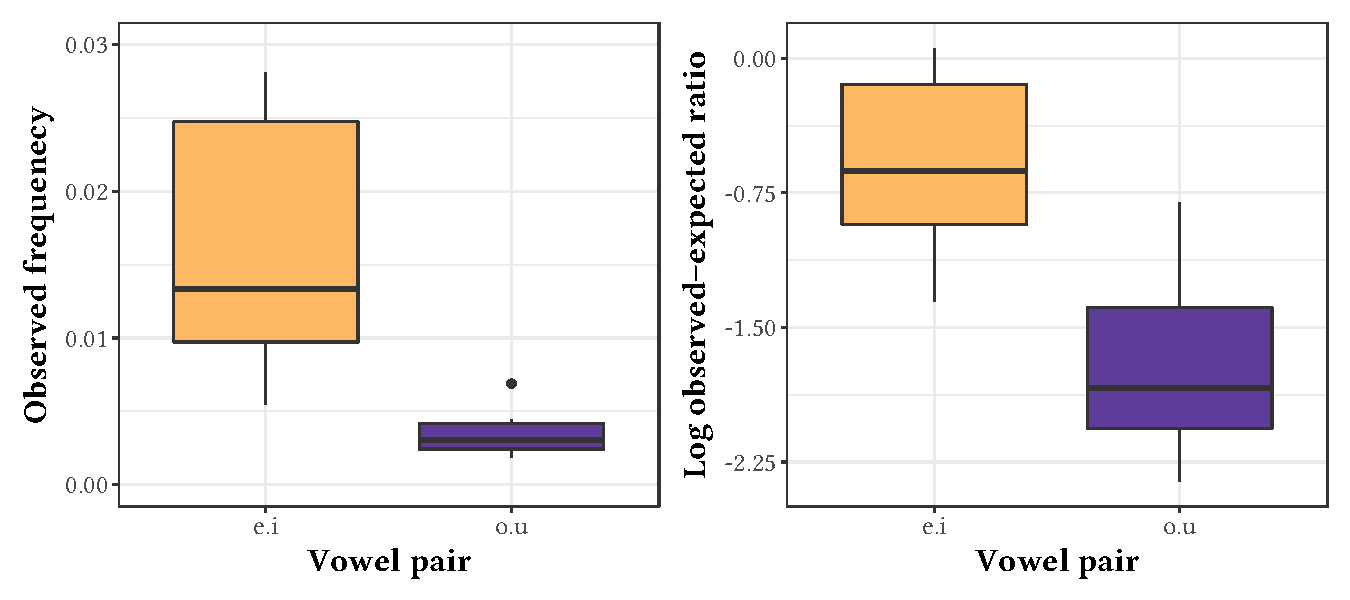
\includegraphics[width=0.875\textwidth]{./figures/eiou-log.pdf}
\end{figure}

Firstly, \autoref{fig:nichols:eeei} shows the clear difference across the sample in the incidence of [e.e] and [e.i] in nouns. Likewise, \autoref{fig:nichols:oou} demonstrates the similar but starker disparity between [o.o] and [o.u] that recurs in each language. \autoref{fig:nichols:eiou} shows that, when comparing [e.i] and [o.u] in these six languages, the latter occurs in nouns at a noticeably lower rate than the former. Lastly, comparing \autoref{fig:nichols:eeei} with \autoref{fig:nichols:oou} shows that overall the difference in nouns between [o.o] and [o.u] is starker than between [e.e] and [e.i].

The analysis also revealed that, in nouns, back rounded [o.u] was the least common of the 25 possible vowel pairs in all six of the sample languages. This was despite the fact that [o.u] was not the vowel pair expected to be the most infrequent in any language in the sample (range 20--23; mean 21.83; median 22; standard deviation 1.17).

Front unrounded [e.i], however, varied in nouns between a rank of 13 in Kalanga and 24 in Yao (mean 20.67; median 22; standard deviation 4.03). Nonetheless, [e.i] was found to have a lower rank than expected in 5 of the 6 languages, with the sole exception being Kalanga.

\section{Discussion}
\begin{sloppypar}
The first point to be acknowledged is that the under-representation of [e.i] and [o.u] and the corresponding over-representation of [e.e] and [o.o] in nouns, where alternations are absent, mirrors what is found in a great many five-vowel Bantu languages in verbs, where harmony can be seen to induce alternations.
\end{sloppypar}

Before discussing this any further, a related aspect of the results (especially as demonstrated by \autoref{fig:nichols:ratio}) must first be addressed. This is the fact that the results do not conclusively demonstrate whether or not the harmony system of a given language, in particular the presence -- as in Chewa, Kalanga, Pende and Yao -- or the absence -- as in Lozi and Makhuwa -- of front height harmony in verbs, has an influence -- direct or not -- on the frequencies of [e.e] and [e.i] in nouns.

In both canonical Kalanga and non-canonical Lozi, [e.i] occurs at roughly the level we would expect given random combination. However, in Kalanga [e.e] is far commoner than [e.i]. This is not the case in Lozi, where [e.e] occurs with similar frequency to [e.i], being only marginally more represented. Nevertheless, this pattern is not replicated in Makhuwa, which also lacks front height harmony but matches more closely the observed--expected ratios of, for example, Pende (which of course does exhibit a form of front height harmony).

This having been noted, the patterns seen when comparing [e.e] with [e.i] and [o.o] with [o.u] in Chewa, Kalanga, Yao and Pende and when considering the difference between the frequencies of [o.o] and [o.u] in Lozi and Makhuwa could perhaps be interpreted as a gradient counterpart in nouns to the categorical rule in verbs. This interpretation would be comparable to \citeauthor{Martin11}'s \citeyearpar{Martin11} observations that, in English, geminates -- which are prohibited tautomorphemically -- are relatively under-represented in heteromorphemic items and that, in Navajo, where sibilants co-occurring within roots must agree for anteriority, compound words containing sibilants disagreeing in anteriority are likewise found less frequently than expected. On the basis of these data, \citet{Martin11} argues that such lexical biases arise as a compromise brought about by the competition between certain phonotactic preferences and semantic preferences.

\citet{Archangeli12a, Archangeli12b} -- which employed a substantially similar methodology to this paper and whose sample of six canonical five-vowel Bantu languages included Chewa, Kalanga and Yao -- have also commented on the patterns of frequency found in nouns as compared to verbs. They suggest that patterns such as those observable in Chewa could be argued to be predictable simply on inductive grounds. Thus, arguing against Universal Grammar (UG) and in a favour of Emergent Grammar (EG), \citet[214]{Archangeli12b} assert that ``UG predicts an absence of an extension while EG predicts extension due to the attractor effect.''\footnote{The ``attractor effect'' being the ``the gradual generalization of an effect to broader classes'', such as the potential spread of vowel height harmony in verbs to nouns \citep[198]{Archangeli12b}.}

However, as \citet[757]{Martin11} acknowledges when considering comparable patterns in tauto- and heteromorphemic contexts in English and Navajo, such distributions ``could both result from the same phonetic pressure''. This is something akin to the notion of ``rule scattering'' (\citealt{RBO15} after \citealt{Robinson76}). In other words, it may instead be that rather than one part of the lexicon exerting an influence over another, both share a common cause.\footnote{For example, the results of the present study might be taken to suggest that the under-representation of [e.i] and [o.u] is due to the well-groundedness of their avoidance because of differences in height and that there is some sort of stronger bias against [o.u] than [e.i] (cf. however, \citealt{Archangeli12b} who failed to find similar consistent effects in a sample of non-Bantu languages).} In the case of English, the same pressure that gave rise to a prohibition on geminates within a morpheme also had a hand in guiding the competition in the lexicon between compounds containing geminates and those lacking geminates.

Recall also that, as noted above and as can be seen in \autoref{fig:nichols:ratio}, Makhuwa, which lacks front-vowel alternations, also displays a marked difference between [e.e] and [e.i] in nouns. Therefore, in this particular instance at least, this cannot be due to the influence of the effect of harmony in verbs.

Moreover, it is potentially problematic for such accounts that [o.u] is much more under-represented than expected in nouns than [e.i] considering that, in four of the six sample languages, both pairs of vowels occur in extremely low levels in verbs. Thus, as [e.i] and [o.u] behave similarly in verbs in languages with both front and back height harmony, a difference in their behaviours in nouns is unexpected. This is also further reflected in a more widely cross-Bantu context by the fact that there appear to be no -- or at least vanishingly few -- cases of Bantu languages that possess front height harmony but lack back height harmony \citep[245]{Hyman99}.

\section{Conclusion}

In this study of six Bantu languages possessing a five-vowel inventory, I examined vowel-pair frequencies in nouns with a particular focus on [e.e]--[e.i] and [o.o]--[o.u], and considered the results of these pairs in relationship with alternations seen in verbs due to vowel height harmony.

The results show that [e.e] and [o.o], which agree in height, are generally over-represented in nouns and that [e.i] and [o.u], which correspondingly disagree in height, are generally under-represented. It was also found that the overall difference in representation of [o.o] compared with [o.u] was greater than the difference between [e.e] and [e.i]. Additionally, the back rounded pair [o.u] is without exception less frequent than front unrounded [e.i] in the current sample. This then suggests that, although there is pressure to avoid both [e.i] and [o.u], this pressure is greater regarding [o.u] than [e.i]. As for the effect of the harmony system, in three of the four languages with front height harmony [e.i] was under-represented in nouns but this was only found in one of the two languages in which front height harmony is absent.

Future work will widen the scope of this study to look at other vowel pairs that are integral to the vowel harmony systems of the Bantu language, such as [e.u] which is an important pair when considering the asymmetric manifestation of harmony in Chewa and other canonical languages. It would also be desirable not only to look at particular languages in closer detail but also to investigate a larger sample of Bantu languages and also expand out of the Bantu family, looking at a larger typologically-balanced sample, to determine whether there is any broader cross-linguistic tendency for the languages to follow patterns similar to those observed in the data presented here.

\section*{Acknowledgements}

I would like to thank Wendell Kimper and Ricardo Bermúdez-Otero for supervision, Stefano Coretta for useful discussion, the audience at the 50\textsuperscript{th} Annual Conference on African Linguistics in Vancouver, Canada for their questions and feedback as well as editor Laura Downing and the two reviewers of this paper for their corrections, criticisms and suggestions. Any shortcomings present in this work are my own.

{\sloppy\printbibliography[heading=subbibliography,notkeyword=this]}
\end{document}
